\subsection{Svorių bei poslinkio patikrinimo funkcija}
\label{subsec:check_accuracy}

Funkcijos veikimo principas (žr.~\ref{fig:check_accuracy_function} pav.):
\begin{enumerate}
    \item Gauname perceptrono skaičiavimo rezultatus.
    \item Grąžinama \textit{True}, jeigu perceptrono apskaičiuotų reikšmių tikslumas yra $100\ \%$ visais kitais atvejais – netiesa (angl.~\textit{False}). 
\end{enumerate}

\begin{figure}[H]
    \centering
    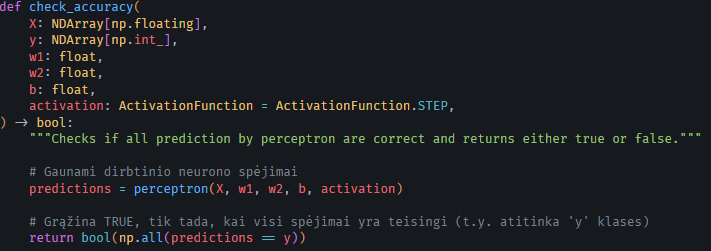
\includegraphics[width=0.75\linewidth]{1Lab/overleaf/images/check_accuracy.png}
    \caption{Svorių bei poslinkio tikrinimo funkcija}
    \label{fig:check_accuracy_function}
\end{figure}